\documentclass{beamer}
%\documentclass[handout,t]{beamer}

\batchmode
% \usepackage{pgfpages}
% \pgfpagesuselayout{4 on 1}[letterpaper,landscape,border shrink=5mm]

\usepackage{ctex,amsmath,amssymb,enumerate,epsfig,bbm,calc,color,ifthen,capt-of}
\usepackage{url} 
\usepackage{hyperref} 
\usepackage{geometry}

\usetheme{Berlin}
%\usecolortheme{mit}

\title{媒体云转码的演进:\\\Small{MapReduce、DASH与稳定婚姻}}
\author{Alan Zhuang\\
\href{mailto:cheedoong@acm.org}{\nolinkurl{cheedoong@acm.org}}\\
}
\date{\today}
\pgfdeclareimage[height=0.25cm]{mit-logo}{tencent_alpha.png}
\logo{\pgfuseimage{mit-logo}\hspace*{0.1cm}}

%\setlist[itemize]{noitemsep}

\AtBeginSection[]
{
\begin{frame}<beamer>
\frametitle{Outline}
\tableofcontents[currentsection]
\end{frame}
}
\beamerdefaultoverlayspecification{<+->}
% -----------------------------------------------------------------------------
\begin{document}
% -----------------------------------------------------------------------------

\frame{\titlepage}

\section[Outline]{}
\begin{frame}{Outline}
\tableofcontents
\end{frame}

% -----------------------------------------------------------------------------
\section{背景}
\subsection{}
\begin{frame}{多屏时代的挑战}
\begin{itemize}
%\pause
\item 多种平台\\ %\pause
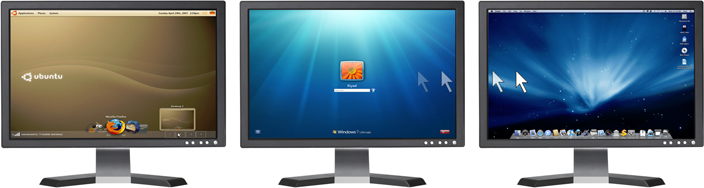
\includegraphics[height=1.6cm]{fig/PCs.png}\pause
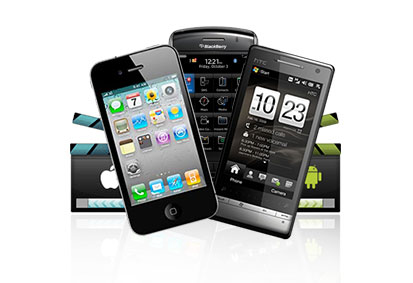
\includegraphics[height=1.0cm]{fig/mobile-bc.png}\pause
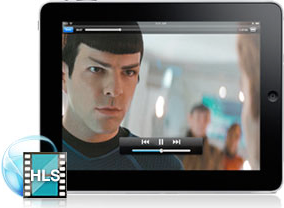
\includegraphics[height=1.1cm]{fig/streaming-bc.png}\pause

\includegraphics[height=1.6cm]{fig/video_quality-bc.png} \pause
\item 多种屏幕大小\\ %\pause
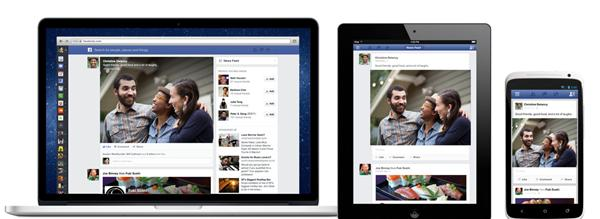
\includegraphics[height=1.2cm]{fig/screen_sizes.jpg}\pause
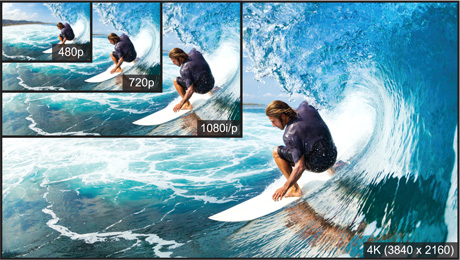
\includegraphics[height=2.2cm]{fig/480_to_4KVideo.jpg}\pause
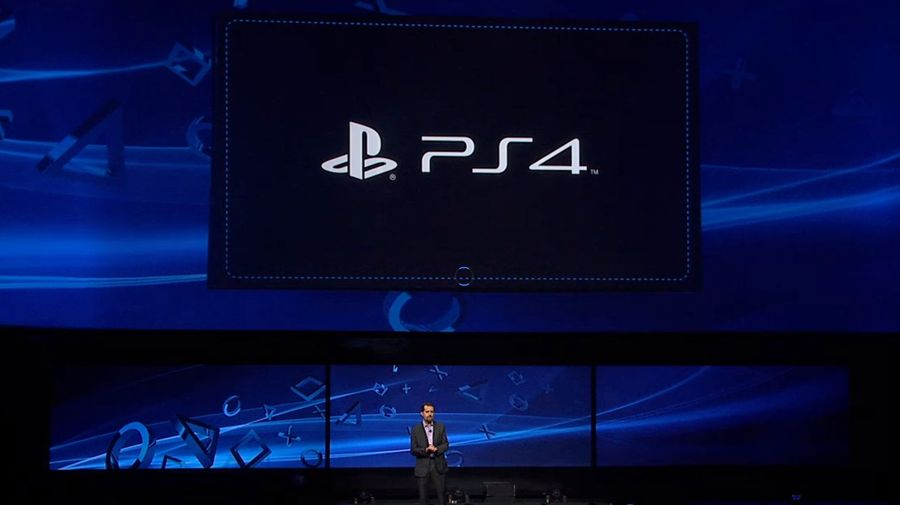
\includegraphics[height=2.2cm]{fig/4k_video.jpg} \pause
\end{itemize}
\end{frame}
\begin{frame}{多屏时代的挑战} 
\begin{itemize}
\item 多种码率\\ %\pause
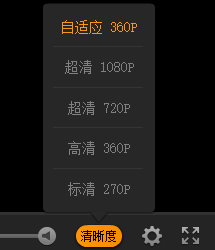
\includegraphics[height=1.9cm]{fig/bitrate_tencent.png}\hspace*{0.4cm}\pause
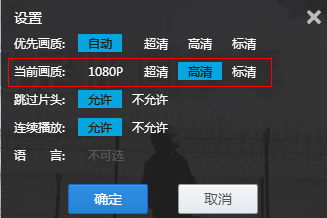
\includegraphics[height=1.9cm]{fig/bitrate_youku.png}\hspace*{0.4cm}\pause
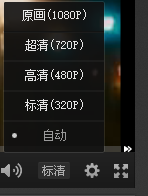
\includegraphics[height=1.9cm]{fig/bitrate_sohu.png}\hspace*{0.4cm}\pause
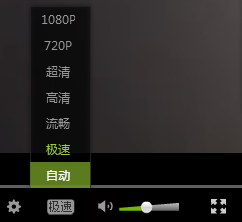
\includegraphics[height=1.9cm]{fig/bitrate_qiyi.png}\pause   
\item 多种解码能力\\ %\pause
%\begin{table}
{\scriptsize
\begin{center}
\begin{tabular}{l|llll} %\toprule
\hline
联发科芯片& MT6572 & MT6582 & MT6588 & MT6592 \\ %\midrule
\hline
Display  & 960$\times$540P & 1280$\times$720P & 1920$\times$1280P & 1920$\times$1280P \\
H.264 Decode   & 720P@30fps & 1080P@30fps  & 1080P@30fps  & 1080P@30fps \\ 
HEVC Decode   &  N/A &  N/A  & 720P@30fps  & 720P@30fps \\ 
\hline
%\bottomrule
\end{tabular}
}
\end{center}
%\end{table}
\end{itemize}
\end{frame}
\begin{frame}{多屏时代的挑战} 
\begin{itemize}
\item 不同封装容器支持\\ %\pause
mp4, mkv, avi, flv, wmv, rmvb, webm, mpeg-ts... \pause
\item 不同编码标准支持\\ \pause
H.264(AVC), H.265(HEVC), VC-1, AVS, VP8/9, RealVideo...
\pause
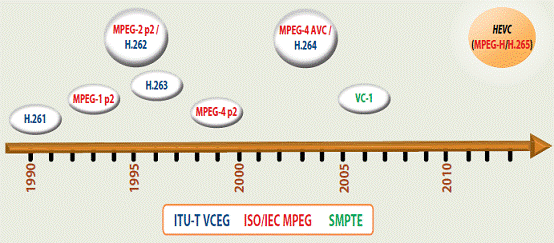
\includegraphics[height=3.5cm]{fig/encoding_standards.png}\pause
\end{itemize}
\end{frame}
\begin{frame}{多屏时代的挑战} 
\begin{itemize}
\item 巨头角力\\ %\pause
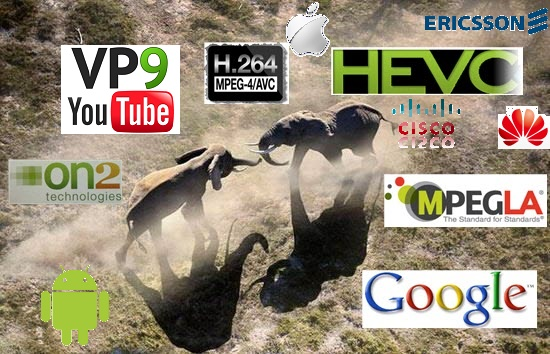
\includegraphics[height=5cm]{fig/competition.jpg}\pause
\end{itemize}
\end{frame}
\begin{frame}{幸运的是,}
\pause
决大多数设备都支持:
\pause
\begin{itemize}
\item 编码标准\\ \pause
H.264/AVC (ISO/IEC 14496-10;  ITU-T H.264; MPEG-4 Part 10).
\item 封装容器\\ \pause
MP4 (ISO/IEC 14496-14; MPEG-4 Part 14).
\end{itemize}
\pause
所以,我们需要把用户/编辑上传的各种不同封装、不同编码的,一般码率比较高的源视频转成若干种适合不同设备的不同码率的H.264编码、MP4封装的视频。
\end{frame}
\begin{frame}{但是,}
\pause
\begin{itemize}
\item 媒体转码是件及其消耗计算资源的工作\\ %\pause
	尤其视频编码,对于目前常见的支持SSE4指令集的x86/x64 CPU的机器:
	\begin{itemize}
	\item  编码H.264视频需要耗费播放时长的1/3到2/3
	\item  编码H.265视频需要耗费播放时长的30+倍
	\item  单个CPU核通常最多可跑1--2个编码任务
	\end{itemize}
\item 媒体文件大,再加上多码率副本,极其消耗存储
\item 潜在的带宽消耗
\end{itemize}
\end{frame}

\begin{frame}{解决}
\pause
Criteria: \pause
\begin{itemize}
\item 单机内\\
	\begin{itemize}
	\item 功能划分、数据局部性\\
	宏块组粒度的并行
	\item 内存访问、CPU核心/Cache拓扑结构和转码格式\\
	帧级或GOP(图像组)级并行\\
	对NUMA机器特别友好
	\end{itemize}
\item 分布式转码
	\begin{itemize}
		\item 存储
		\item 路由
		\item 任务调度
	\end{itemize}
\end{itemize}
\end{frame}

% -----------------------------------------------------------------------------
\section{从Cloud Transcoder到TranscX}
\subsection{前腾讯研究院Cloud Transcoder}
\begin{frame}{前腾讯研究院Cloud Transcoder}
\textbf{Done 2011-. Gale Huang et al. Cloud transcoder: bridging the format and resolution gap between internet videos and mobile devices. ACM NOSSDAV 2012.}\\\pause
\begin{center}
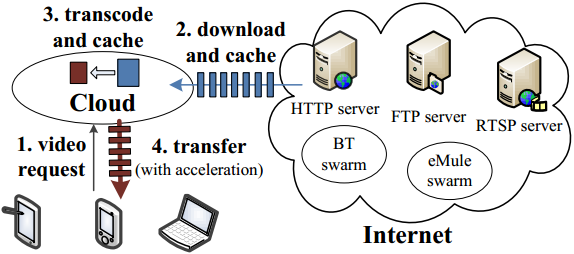
\includegraphics[height=2.8cm]{fig/clouder-transcoder_principle.png}\\\pause

\includegraphics[scale=0.36]{fig/cloud_transcoder_nossdav_affiliation.png}
\end{center}
\end{frame}

\begin{frame}
\begin{center}
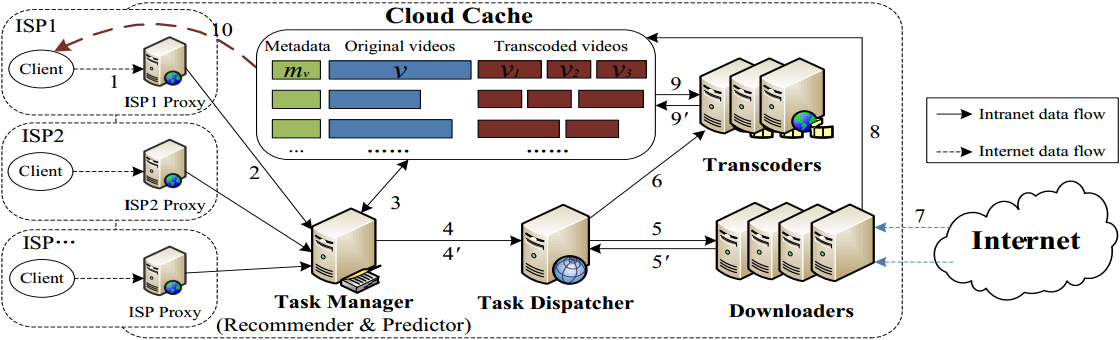
\includegraphics[width=11.5cm]{fig/cloud-transcoder_arch.png}
\end{center}
\end{frame}
\begin{frame}
\begin{center}
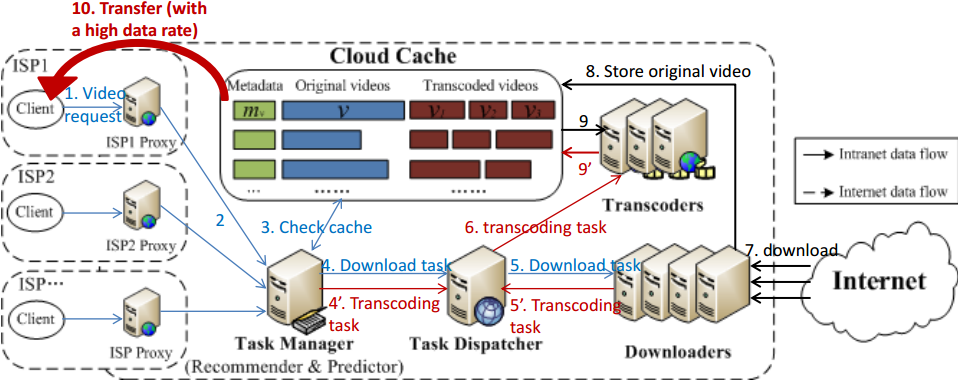
\includegraphics[width=11.5cm]{fig/cloud-transcoder_arch_details.png}
\end{center}
\end{frame}
\begin{frame}
\begin{center}
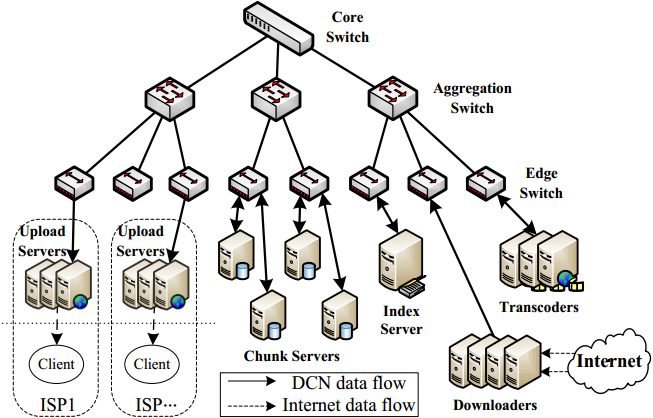
\includegraphics[width=10cm]{fig/cloud-cache_hardware.png}
\end{center}
\end{frame}
\subsection{架平流媒体TranscX}
\begin{frame}{架平流媒体TranscX}
TranscX: 
\begin{itemize}
	\item Transcoding eXpress/eXperience/eXtreme...; transc(x)
\end{itemize}
\begin{center}
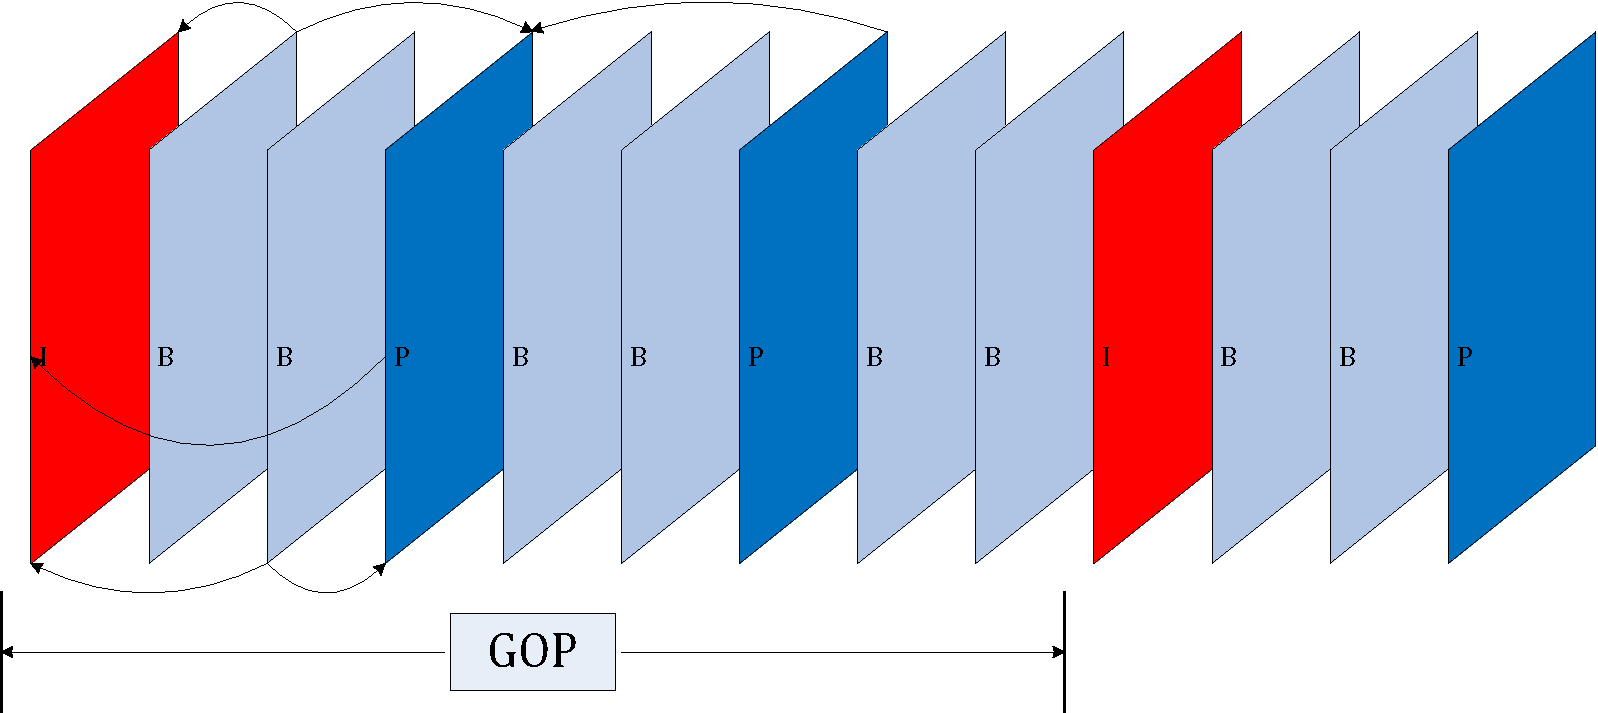
\includegraphics[scale=0.20]{fig/GOP.pdf}
\end{center}
\begin{itemize}
\item GOP-level parallelism without REAL splitting\\
Media head parsing, $<begin\_time, end\_time> or GOP\_id \rightarrow <start_offset, size>$
\end{itemize}
\end{frame}
\begin{frame}
\begin{itemize}
\item Job/Map/Thread, accurate control and CPU \& I/O limitation
\item Real-time support for DASH and Live Broadcasting
\item Migration from Computing to Storage: soul of cloud tech
\item It later supported WeChat, Qzone and Weishi
\item 用MapReduce框架统一了起来,减少了调度的复杂性,增强了可扩展性
\item 复用了存储服务器的空间计算资源,节省了成本
\end{itemize}
\end{frame}

\begin{frame}
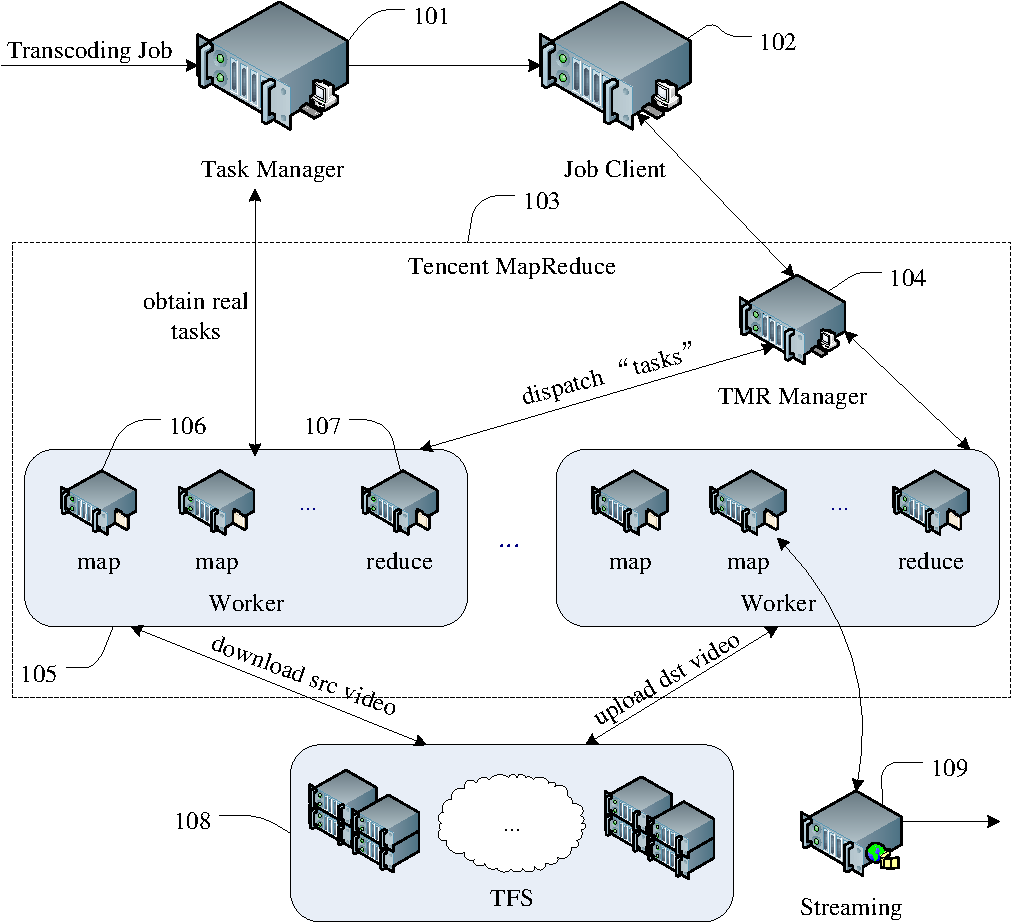
\includegraphics[scale=0.33]{fig/TranscX.pdf}\hspace*{0.1cm}
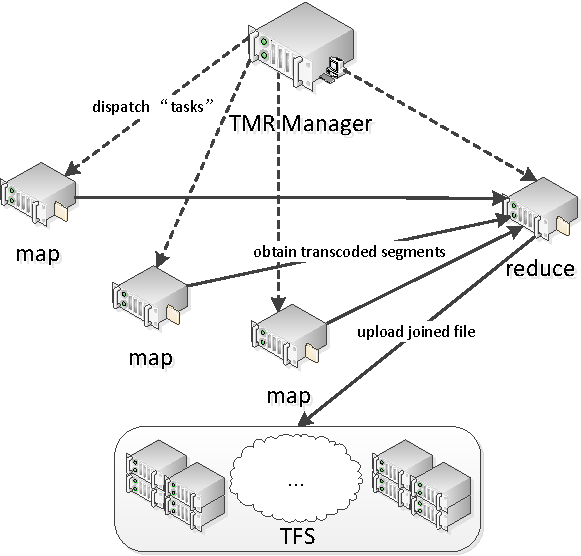
\includegraphics[scale=0.33]{fig/TranscX_detail.pdf}
\end{frame}

\section{DASH与稳定婚姻}
\subsection{DASH}
\begin{frame}{Why DASH?}
DASH: Dynamic Adaptive Streaming over HTTP.
\pause
\begin{itemize}
\item 庞大的文件头,导致在线播放时较大的initial/VCR delay
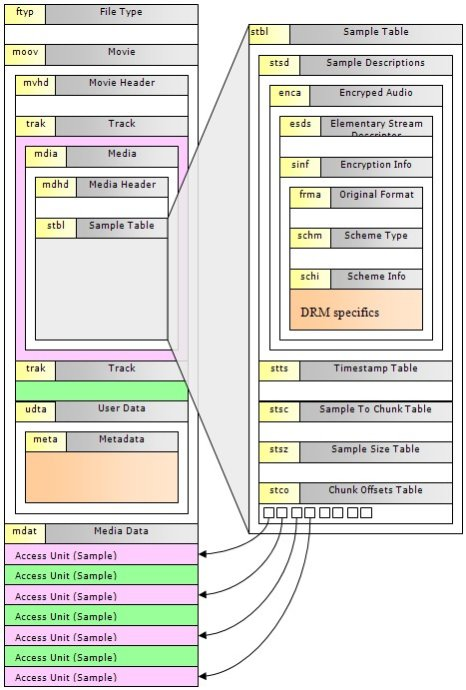
\includegraphics[height=4cm]{fig/MP4_boxes_detail.jpg}
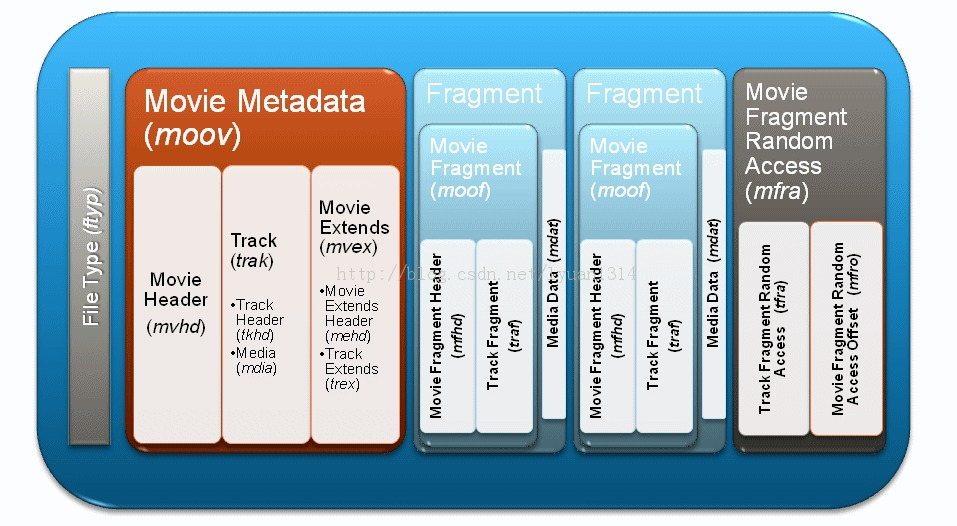
\includegraphics[height=4cm]{fig/fragmented_mp4.jpg}
\end{itemize}
\end{frame}
\begin{frame}
\begin{itemize}
\item 非平滑的码率间切换 due to varying download speed
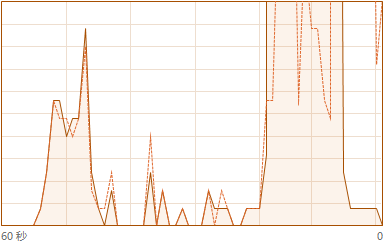
\includegraphics[height=4.5cm]{fig/download_speed.png}
\end{itemize}
\end{frame}
\begin{frame}{DASH}
DASH: Dynamic Adaptive Streaming over HTTP. \\
几种DASH标准:
\pause
\begin{itemize}
\item Apple HLS (HTTP Live Streaming) 2009
\item Microsoft HSS (HTTP Smooth Streaming) 2010
\item Adobe HDS (HTTP Dynamic Streaming) 2010
\item MPEG-DASH (ISO/IEC 23009-1) 2012
\end{itemize}
\end{frame}
\begin{frame}{Apple HLS}
\begin{itemize}
\item Architecture
\begin{center}
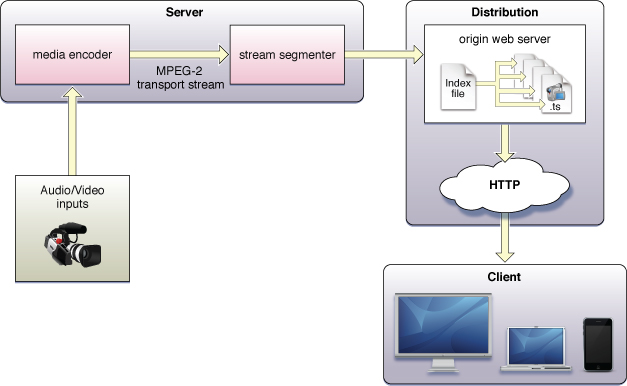
\includegraphics[height=4.5cm]{fig/hls_arch.jpg}
\end{center}
\end{itemize}
\end{frame}
\begin{frame}{Apple HLS}
\begin{itemize}
\item Segment Indexing
\begin{center}
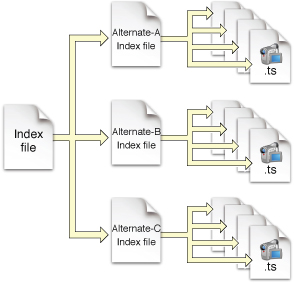
\includegraphics[height=4.5cm]{fig/hls_indexing.jpg}
\end{center}
\end{itemize}
\end{frame}

\begin{frame}{MPEG-DASH}
\begin{itemize}
\item Architecture
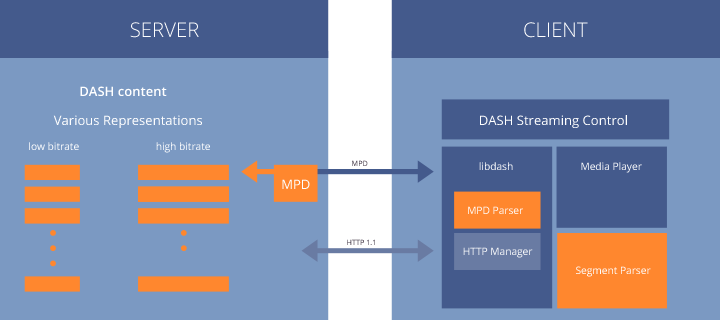
\includegraphics[height=4.5cm]{fig/MPEG-DASH_arch.png}
\end{itemize}
\end{frame}
\begin{frame}{MPEG-DASH}
\begin{itemize}
\item Data Model
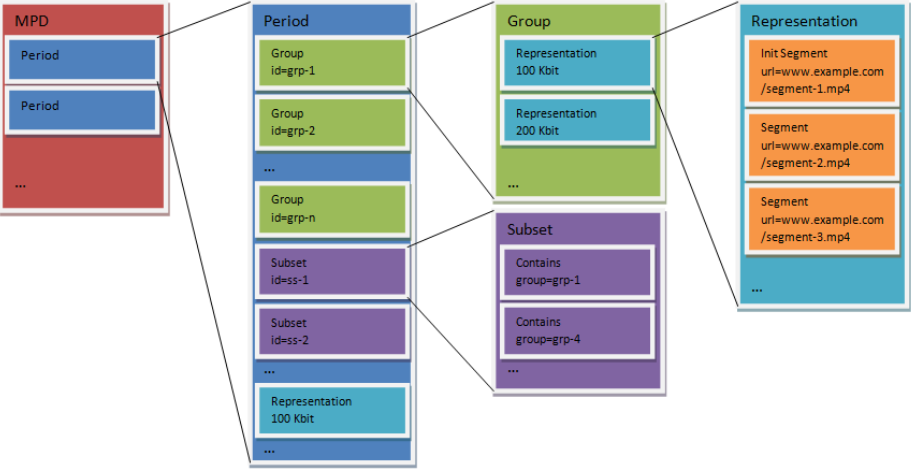
\includegraphics[height=4.5cm]{fig/mpeg-dash_data_model.png}
\end{itemize}
\end{frame}
\begin{frame}{MPEG-DASH}
\begin{itemize}
\item Segment Indexing
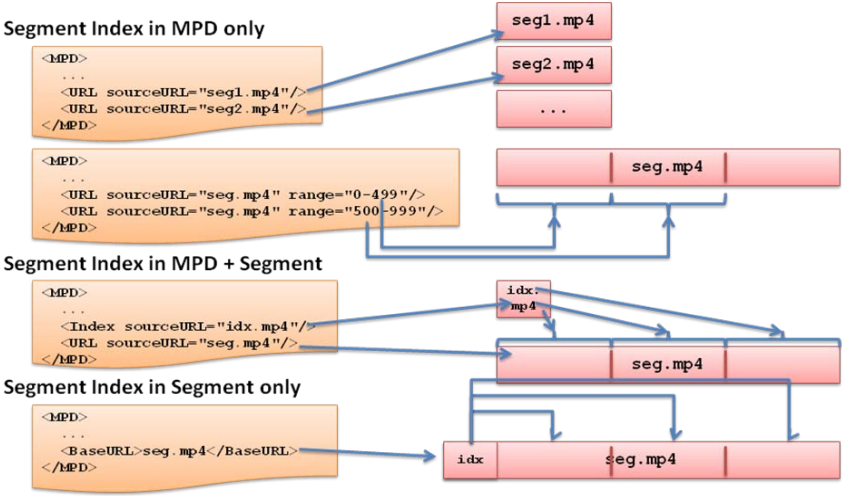
\includegraphics[height=5cm]{fig/mpeg-dash_indexing.png}
\end{itemize}
\end{frame}

\begin{frame}{架平流媒体对DASH的使用}
\begin{itemize}
\item 尽量只转封装,不转编码
\item 实时、按需转封装/转码
\item 使用/自写的多种协议,解决并发I/O流少的问题
	\begin{description}
	\item[tmpfs] 最简单、方便,对Cache管理要求不强的场合
	\item[in\_mem] in memory, 进程内的编解码I/O
	\item[shm\_mem] shared memory, 多进程的编解码I/O,可自定义Cache管理、淘汰算法
	\item[AVIOContext] FFMPEG built-in
	\item[async\_http] 适用直播,数据到达不可预期
\end{description}
\item FPGA HEVC Encoding (proposed)
\end{itemize}
\end{frame}

\subsection{稳定匹配}
\begin{frame}{Motivation}
DASH和Wechat, Weishi, Qzone等社交UGC视频转码中存在的问题:
\begin{itemize}
\item 视频长度较短\\
一般仅一个到若干个GOP,MapReduce时仅需要一个Mapper
\item 但MapReduce任务调度的延时较大\\
有时甚至超过播放时长。可通过Linux Container守护进程的实时MapReduce来缓解,但非根本解决之道
\item 大部分视频的未来访问少于X次\\
还有比较全码率转码+全量分发么?
\end{itemize}
\end{frame}
\begin{frame}{Motivation}
%对大数据的分析,得出结论:
\begin{itemize}
	\item 对数千台后台服务器连续一周运行状态的测量:\\
		\begin{itemize}
		\item 不仅DC,OC的多数服务器大部分时间CPU负载也较低\\
		甚至包括某些HTTP服务器
		\item 多数服务器的CPU负载基本不会出现突变\\
		CPU负载随时间相对平稳,但不同地区的平均负载存在差异
		\end{itemize}
	\item 对应时间所有用户访问和调度情况的测量:\\
		\begin{itemize}
		\item 用户对CDN的region选择存在偏好\\
		由于网络拓扑关系,用户去不同的CDN边缘节点下载的速率各不相同,而目前的调度算法,至少能得到一个次优解
		\item 不同不同地区的用户对码率存在偏好\\
		在前面次优解的前提下,不同地区得到平均服务质量有差异
	\end{itemize}
\end{itemize}
\end{frame}

\begin{frame}{优化问题}
\begin{itemize}
\item 选择选择...\\
to be written...
\item 稳定稳定匹配\\
to be written...
\end{itemize}
\end{frame}
\begin{frame}{算法应用}
准备与预测框架\\
\begin{itemize}
\item 用户对所有CDN边缘节点的偏好\\
根据过去的测速数据来Rank用户对所有CDN边缘节点的偏好
\item 每段视频未来一段时间的访问频率\\
根据CDN到用户的带宽和过去一段时间用户的访问频次预测未来一段时间所有有可能有访问的视频的访问频次
\item 未来一小段时间服务器的期望空间计算资源\\
根据分工作日/周末两种自回归模型预测未来一段时间每个OC节点服务器的期望CPU负载
\end{itemize}
\end{frame}

\section{Future Vision}
\subsection{和一些新技术的结合}
\begin{frame}{和一些新技术的结合}
\begin{itemize}
\item WebRTC\\
Client-end caching \& delivery \& broadcasting
\item HTML5 WebSocket, HTTP 2.0\\
会话保持,多流传输
\item Social Could TV\\
\item SVC, MVC, HEVC, NC\\
编码、多副本多版本机制、多视角、传输
\end{itemize}
\end{frame}
\subsection{Acknowledgment}
\begin{frame}{Acknowledgment}
本slides中部分内容源自与以下人员的协作/交流:
\begin{itemize}
\item 架平流媒体\\
Leon Ouyang, Devin Zeng, Guita Zhang, Kernel He, Chris Su
\item Tsinghua-Tencent Joint Lab.\\ 
Zhi Wang
\item SNG社交平台部\\
Stone Huang
\item NTU\\
Young Wen
\end{itemize}
\end{frame}
% -----------------------------------------------------------------------------
\end{document}
